
\documentclass[varwidth=\maxdimen, border=0.2cm]{standalone} 
\usepackage[T1]{fontenc}
\usepackage[utf8]{inputenc}
\usepackage{xcolor}
\usepackage{tikz}
\usepackage{tikz-qtree}
\usetikzlibrary{positioning}

\definecolor{bluish}{HTML}{E0EBF5}
\definecolor{yellish}{HTML}{FFFFA8}
\definecolor{dbluish}{HTML}{375EAB}
\definecolor{brownish}{HTML}{BC8C64}
\definecolor{darkish}{HTML}{6F6B69}
\definecolor{darkish2}{HTML}{848475}




\begin{document}

\begin{center}
 {\large\tt let max $=${} fn(x,y)\{{}if (x$>${}y)\{{}return x\}{} y\}{}} 
\end{center}

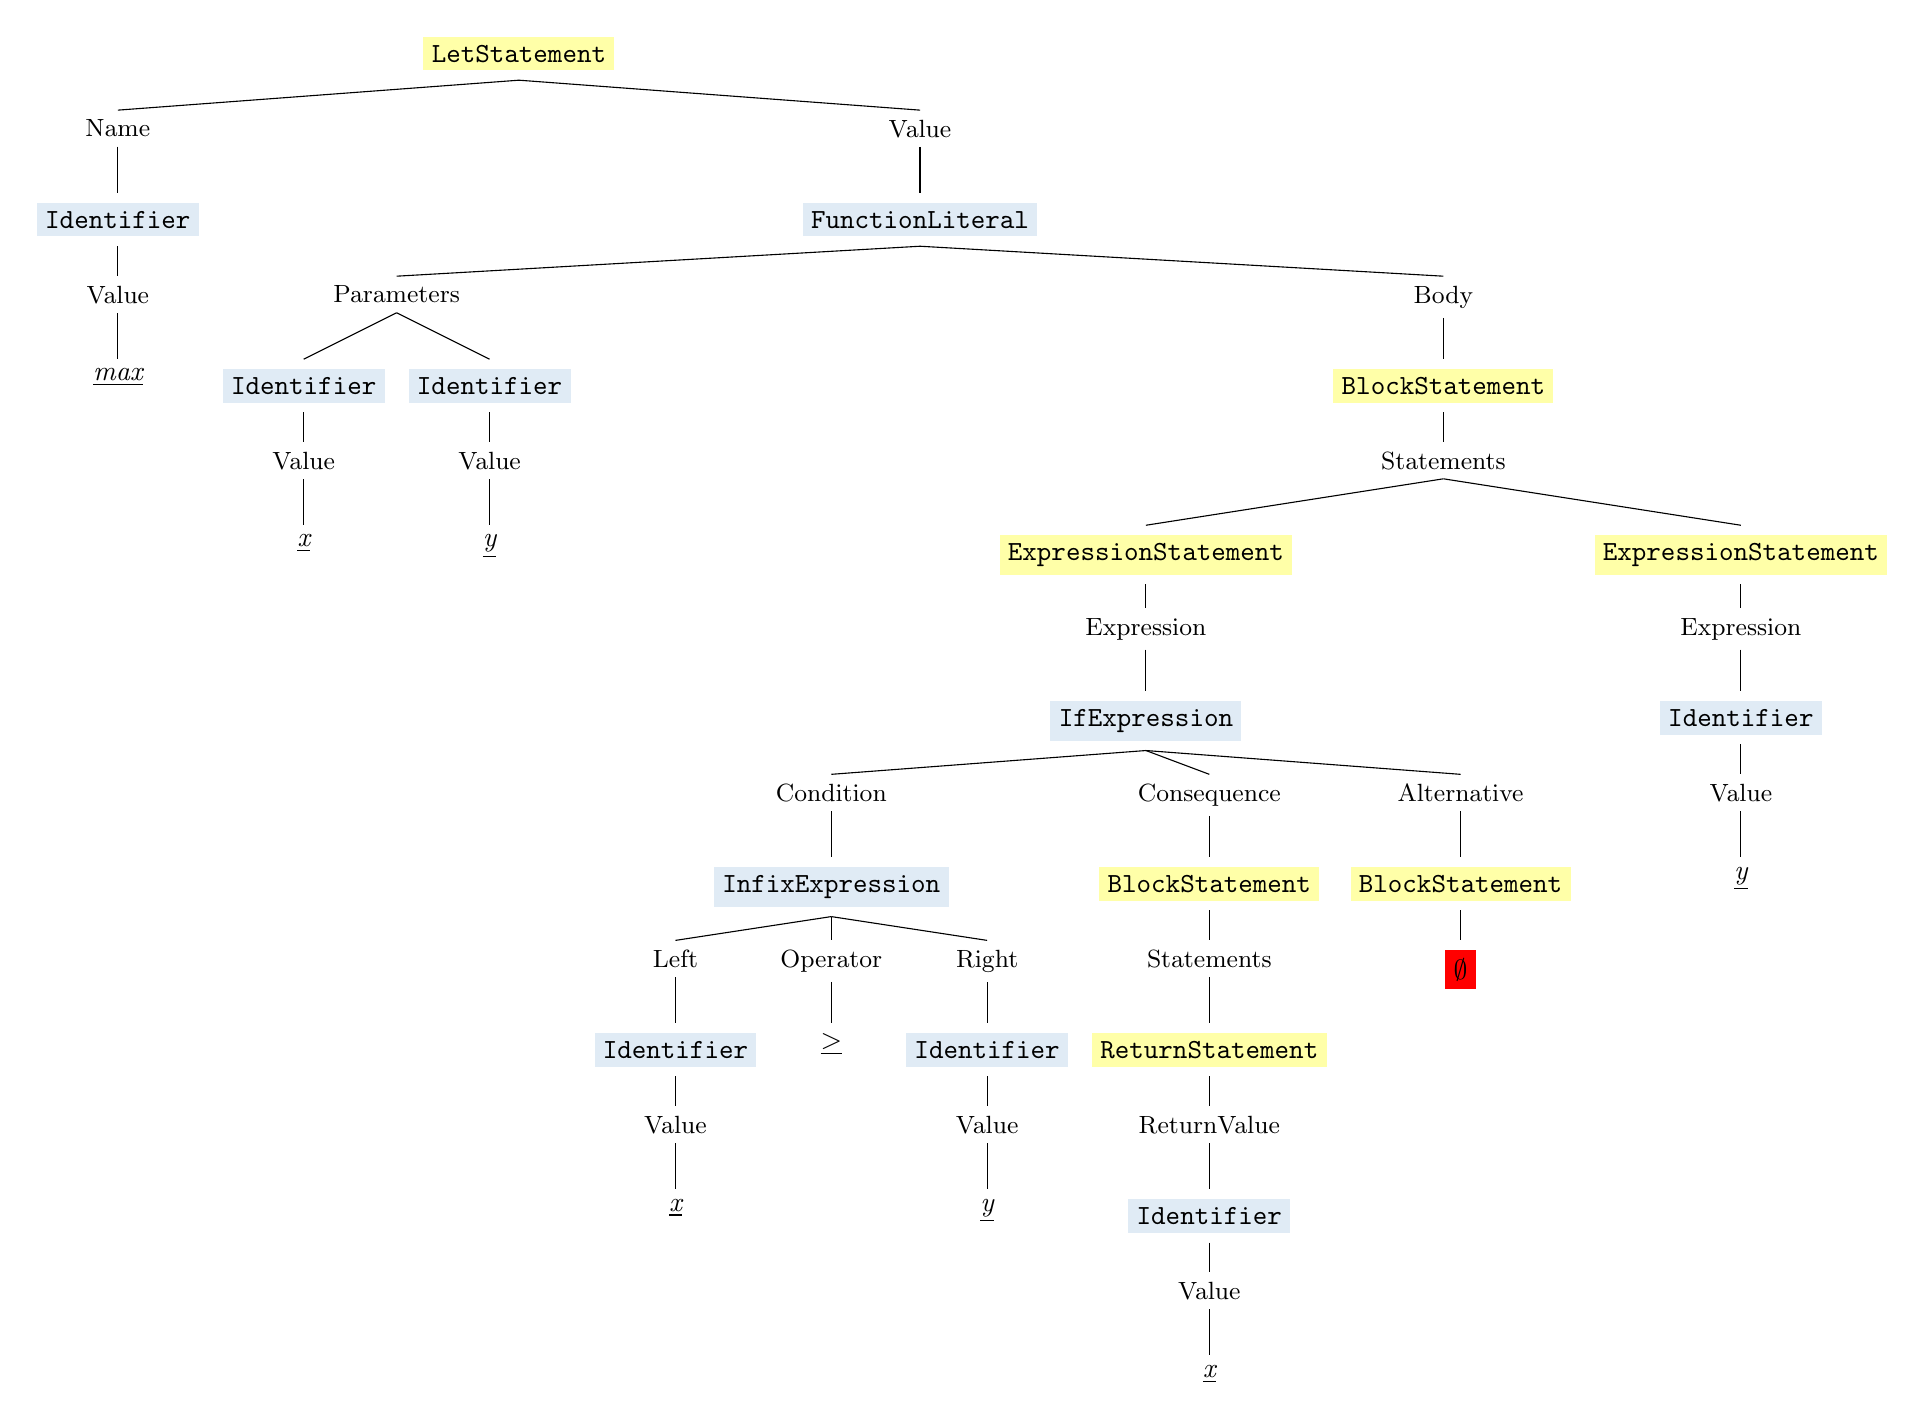
\begin{tikzpicture}[
   every tree node/.style={anchor=north},
   every node/.append style={align=left}  
]

\Tree [.{\colorbox{yellish}{\textcolor{black}{\tt LetStatement}}}
  [.{\small Name} 
    [.{\colorbox{bluish}{\textcolor{black}{\tt Identifier}}}
      [.{\small Value} 
        \underline{\it max}
      ]
    ]
  ]
  [.{\small Value} 
    [.{\colorbox{bluish}{\textcolor{black}{\tt FunctionLiteral}}}
      [.{\small Parameters} 
        [.{\colorbox{bluish}{\textcolor{black}{\tt Identifier}}}
          [.{\small Value} 
            \underline{\it x}
          ]
        ][.{\colorbox{bluish}{\textcolor{black}{\tt Identifier}}}
          [.{\small Value} 
            \underline{\it y}
          ]
        ]
      ]
      [.{\small Body} 
        [.{\colorbox{yellish}{\textcolor{black}{\tt BlockStatement}}}
          [.{\small Statements} 
            [.{\colorbox{yellish}{\textcolor{black}{\tt ExpressionStatement}}}
              [.{\small Expression} 
                [.{\colorbox{bluish}{\textcolor{black}{\tt IfExpression}}}
                  [.{\small Condition} 
                    [.{\colorbox{bluish}{\textcolor{black}{\tt InfixExpression}}}
                      [.{\small Left} 
                        [.{\colorbox{bluish}{\textcolor{black}{\tt Identifier}}}
                          [.{\small Value} 
                            \underline{\it x}
                          ]
                        ]
                      ]
                      [.{\small Operator} 
                        \underline{\it $>${}}
                      ]
                      [.{\small Right} 
                        [.{\colorbox{bluish}{\textcolor{black}{\tt Identifier}}}
                          [.{\small Value} 
                            \underline{\it y}
                          ]
                        ]
                      ]
                    ]
                  ]
                  [.{\small Consequence} 
                    [.{\colorbox{yellish}{\textcolor{black}{\tt BlockStatement}}}
                      [.{\small Statements} 
                        [.{\colorbox{yellish}{\textcolor{black}{\tt ReturnStatement}}}
                          [.{\small ReturnValue} 
                            [.{\colorbox{bluish}{\textcolor{black}{\tt Identifier}}}
                              [.{\small Value} 
                                \underline{\it x}
                              ]
                            ]
                          ]
                        ]
                      ]
                    ]
                  ]
                  [.{\small Alternative} 
                    [.{\colorbox{yellish}{\textcolor{black}{\tt BlockStatement}}}
                      \colorbox{red}{\textcolor{black}{\tt $\emptyset$}}
                    ]
                  ]
                ]
              ]
            ][.{\colorbox{yellish}{\textcolor{black}{\tt ExpressionStatement}}}
              [.{\small Expression} 
                [.{\colorbox{bluish}{\textcolor{black}{\tt Identifier}}}
                  [.{\small Value} 
                    \underline{\it y}
                  ]
                ]
              ]
            ]
          ]
        ]
      ]
    ]
  ]
]
\end{tikzpicture}

\end{document}
